\section{Goals and Architecture}
\label{sec:goals}
In this section, we discuss the motivation for \meddle, describe our goals for the 
system and present an architecture to meet those goals.

\subsection{Motivation}
\meddle is motivated by the fact that users and researchers currently 
have a limited view -- if any -- into how devices and apps generate network 
traffic. In addition, there are few mechanisms available for shaping, modifying 
or blocking this network traffic. 

This can be harmful to users, as apps may generate sufficient traffic
to cause overage charges on cell phone bills. Even when the volume of
traffic is small, a periodic network activity can quickly deplete
battery charge by preventing power management policy of the device to
correctly operate~\cite{qian:periodic}. Further, apps can use the network to leak personal
information or track users without consent~\cite{hornyack:appfence}.

Researchers  likewise suffer from a lack of visibility and control over 
network traffic. It is common 
to use testbeds or proprietary ISP datasets to reveal network usage 
and its impact on data quota, battery life and privacy. However, the 
coverage and representativeness of these results can by limited by 
the use of i) a single carrier's network, ii) a small testbed with 
a single, custom operating system and iii) a single access technology 
(cellular or WiFi). Once researchers identify a problem with network traffic, 
addressing it can be challenging. OS developers are slow to 
adopt changes, app developers may be unwilling to modify their code 
and carriers often have no incentive to deploy new in-network 
functionality. 

%However, there is a large and dynamic set of 
%apps, devices and usage patterns that are not captured in the lab 
%environment. Assuming that such studies reveal pathological control network traffic is similarly limited, as 
%it may require changes to the operating system and to apps.  Even  Without visibility 
%into how apps and devices use the network in the wild, 
%To characterize mobile traffic and design new protocols and
%services that are better tailored to the mobile environment, we would like a
%framework that allows us to intercept and potentially modify traffic
%generated by mobile devices as they move with users, regardless of the
%device, OS or carrier. However, implementing this functionality is
%difficult on mobile devices because it requires warranty-voiding
%techniques such as jail breaking to access and manipulate traffic at
%the network layer~\cite{enck:taintdroid}. Even when using such an
%approach, carriers may manipulate traffic once it leaves the mobile
%device~\cite{wang:middleboxes}, thus rendering some research
%impractical. Last, some protocols and services should be implemented
%in the network instead of the device (e.g., prefetching and security
%filters) but researchers generally have no ability to deploy such
%solutions.

\subsection{System Goals}
The two primary goals for \meddle are 1) to provide comprehensive visibility into 
mobile networking traffic and 2) facilitate the development of new solutions 
and services for mobile networks. We further identify the following sub-goals 
that address limitations of previous work.

\begin{itemize}
\item \emph{Portability.} We want a solution that works regardless of operating system, 
access technology and provider, without requiring advanced (and possibly warranty-voiding) 
techniques such as rooting a phone. 
\item \emph{Pervasiveness.} For maximum transparency, our system should provide seamless 
visibility into all network traffic generated by devices. This means continuous monitoring 
over time and as users move with their devices.
\item \emph{Deployability.} Our solution should be easy to use, immediately deployable 
and incur reasonable costs (or none at all) for users. 
\item \emph{Isolation.} To prevent existing in-network devices from interfering with these new 
solutions and services, our system should provide network-traffic isolation. 
\item \emph{Control.} To enable new solutions and services, our system should enable users and researchers 
to shape, modify or block network traffic. 
\end{itemize}

\subsection{Design and Architecture}

\subsubsection{Design}
To meet the above goals, we propose building a system that redirects all mobile-device 
network traffic to a server outside the carrier's network, thus providing a point of control 
where one can characterize, modify or block this traffic before sending it to the intended 
destination. Importantly, we observe that we can do this today without any additional 
support for devices or carriers: the key idea is to combine software middleboxes (e.g., 
packet filters, proxies, etc.) with virtual private networks (VPNs). 

We use VPNs to achieve our goals of portability, pervasiveness, deployability 
and isolation. Specifically, major
 mobile OSes provide built-in VPN functionality for enterprise
 customers to enable access to resources in
 the enterprise's private network for employees ``on the road". 
In \meddle, we use VPNs as a portable mechanism\footnote{Android, BlackBerry and iOS and Windows 8 all support VPNs natively, representing more than 86\% of the mobile device market\cite{gartner-phone-share}.} to tunnel traffic from mobile devices to a machine outside of the carrier's network for the purpose of analysis and interposition. 

We use software-middlebox techniques to meet the goal of providing control over network traffic in the mobile 
environment~\cite{sherry:middleboxes}. Middleboxes are traditionally used in managed networks (e.g., in enterprises and ISPs) to implement policies and enhanced services over IP. In \meddle, we use middleboxes as a mechanism not only to implement custom policies and services for users and service providers, but also for measuring networks and experimenting with alternative protocols for the mobile environment without requiring access to mobile carrier networks. 

%\tbdal{here it would be good to introduce which VPN technology is
%  used, give a reference to it, explain that it is an open VPN
%  technology (with contrast to a proprietary one that would need
%  vendor specific appliances to work, and claim that this same VPN
%  technology is used by most mobile OSes.}
% \footnote{Vendors such as 
% Cisco and Vyatta also provide implementations that use hardware acceleration.} 

\subsubsection{Architecture}
Figure~\ref{fig:arch} depicts an architectural diagram for how we realize this 
approach via \meddle. Devices use VPN connections to tunnel all 
traffic to one of potentially many \meddle servers. We envision that \meddle 
can run as a single-user system in a user's home network or in a hosted data center, 
or it can run as a shared, distributed and/or virtualized cloud-based service (\eg, on 
Amazon EC2). The 
figure depicts the latter, where multiple \meddle replicas are available for any 
given device. 

\begin{figure}
\centering
        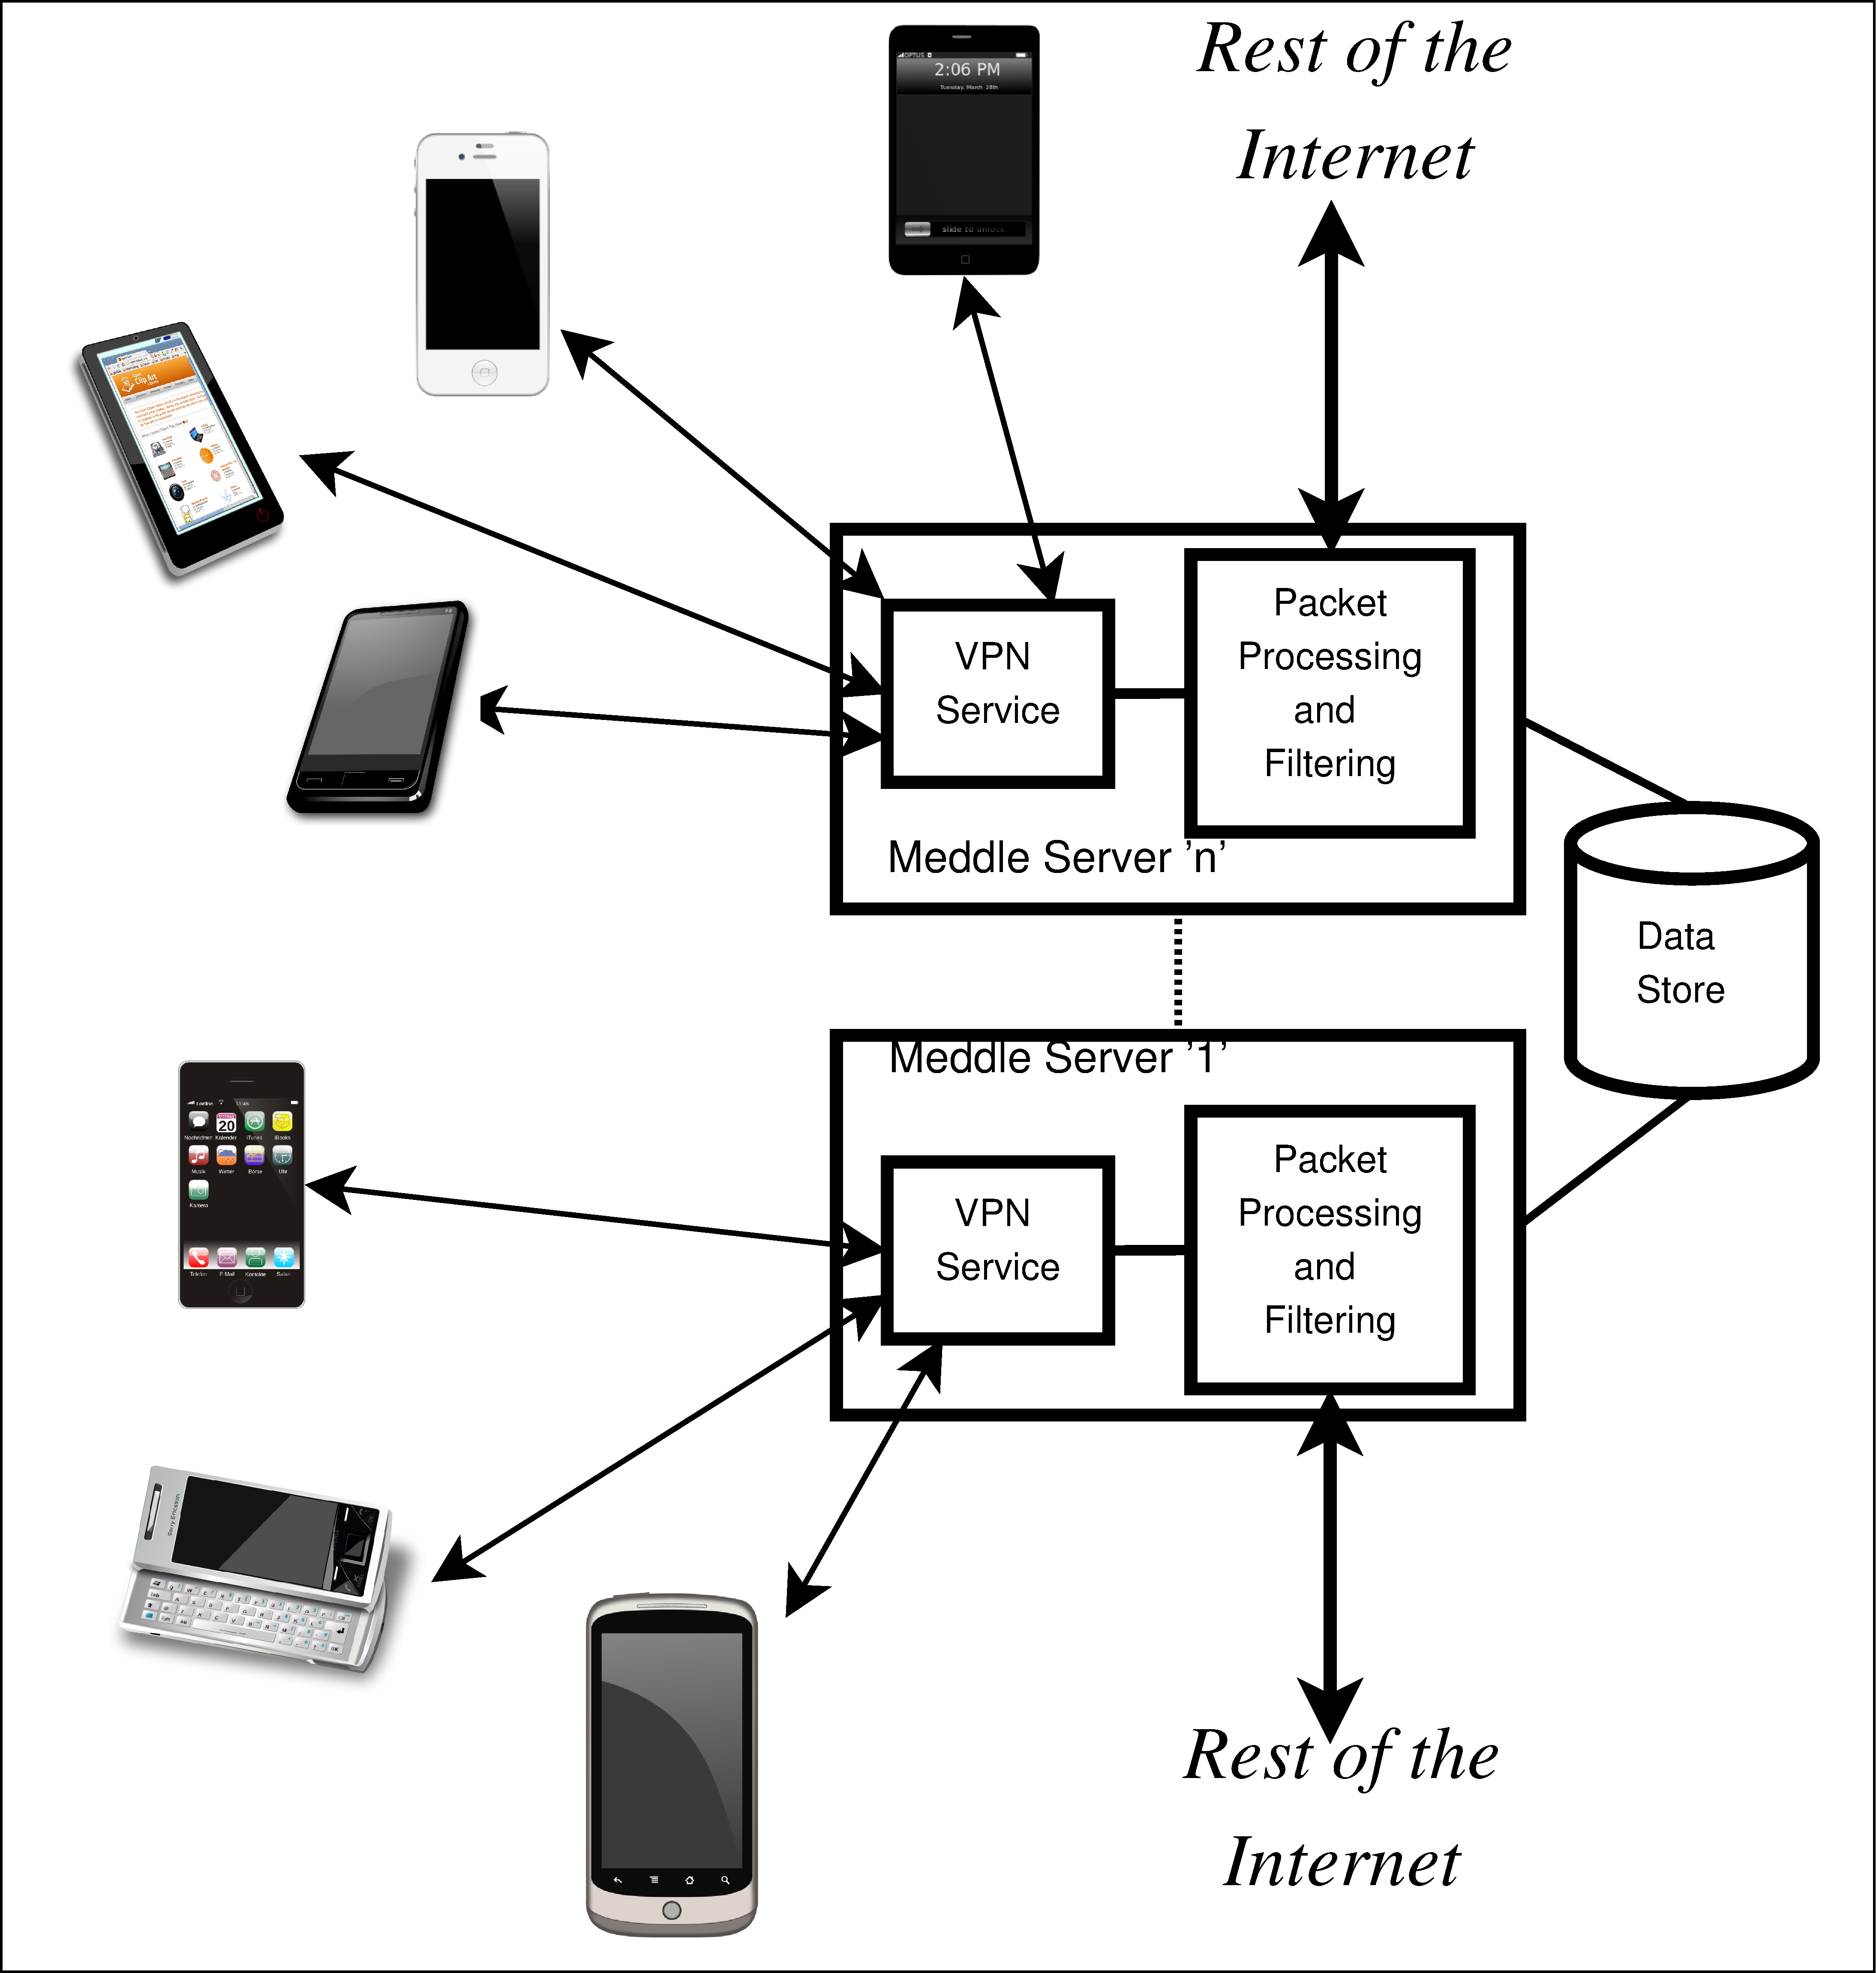
\includegraphics[width=0.8\linewidth]{figs/meddle-servers.pdf}
\vspace{\figcapspace}
  \caption{\meddle architecture. Devices use VPN connections to tunnel all 
  traffic to one of potentially many \meddle servers dynamically chosen to 
  optimize for performance. Each \meddle server uses a device- or user-specific 
  profile to determine the set of services that will operate on the tunnel's network traffic.}
  \label{fig:arch}
\vspace{\postfigspace}
\end{figure}

In the distributed scenario, when a device attempts to connect to \meddle, we direct it to a nearby 
\meddle server in a similar way to how the Akamai CDN uses DNS to redirect 
Web clients to nearby content caches~\cite{akamai:cdn}. 
To optimize for performance, the service can send VPN clients to a 
server that is relatively near the location at which data exits
the mobile carrier's network to enter the Internet. This technique 
can also redirect clients based on server load, reachability and availability. 

To meet the goal of providing control over network traffic in the mobile 
environment, each \meddle
server uses software-middlebox techniques, or \emph{meddleboxes} to interpose on 
network traffic. These meddleboxes can (i) implement custom services for users such as packet
filtering, caching, and intrusion detection, (ii) monitor network
traffic characteristics, and (iii) allow us to experiment with alternative
algorithms and protocols for the mobile environment.
The system maintains a per-device and per-user profile 
to determine the set of services that will operate on the tunnel's 
network traffic. 

Meddleboxes are monolithic in our current implementation, meaning 
that all meddlebox features are within the same \meddle server. When deployed 
in the cloud and at scale, this could lead to suboptimal scaling because 
users might adopt meddlebox features unevenly. To address this, we are 
developing a cloud-based distributed meddelbox deployment where each service runs 
in its own virtual machine (VM) and a user's traffic is routed through a series of these VMs using a 
software-defined network to set up per-user routes on demand.

While the \meddle architecture is straightforward, there are a 
number of challenges we must address in building a viable deployment. 
In the next section, we describe how we achieve continuous monitoring 
of network traffic across platforms, then demonstrate that the power, data-volume and latency 
overheads are reasonably small.







%DRC: These are the things I think we need to emphasize as key features
%
%Portable (Cross platform, access technology, provider w/o needing app or rooting)
%Continuous/Pervasive (always on)
%Passive (low cost, real traffic)
%Control


% - Increase transparency of the opaque mobile ecosystem
%   + Opaque because
%     - tied to OS, service provider
%     - limited knowledge of apps - measurement studies limited to small user set or data sets from cell providers
%     - no knowledge of what service providers are doing
%       - Trip wire 
%     - only way to address somes of these issues is to root the phone, but this cannot shed light on what carriers are doing
%   + Allow users to ensure they are getting what they pay for
%   + Prevent and/or monitor carrier interference
%   + Understand network footprint of apps and devices over time
% - Expose control knobs to enable users to tune the traffic 
%   + Control knobs exists on home gateways and people use it (DRC: Not sure we can prove anything about this)
%      - Firewalls on home gateways but none for mobile - direct exposure to internet 
%	DRC: This isn't true. Mobile networks are in a sense a giant firewall.
%      - Control knobs to filtering traffic given by iOS but details not publicly available (DRC: Mainly, these knobs are coarse-grained and insufficiently expressive to meet the intended goals of parental controls.)
% - Have a low barrier to entry
%   + Users do not want to violate terms of service (DRC: They want to, but are afraid to :-)
%   + Rooting/Jailbreaking issues - not easy, ROMs may not be available for device, opens device to huge security risks
% - VPN based middleboxes to achieve each of these goals
%** System Descripton
% - VPN based middlebox
%    - Why VPNs and advantages of VPNs 
%      + comprehensive view -- cross access technology, service provider, device
%      + native IPsec support on smartphones and tablets
%      + low barrier to entry -- no need to jailbreak phone or install custom OS
%    - - Summary
%    - We need strong statements here to indicate this is indeed feasible
%    - We can cancel the affects of these overheads by the value added services that we provide
